\documentclass{report}
\usepackage{graphicx}


\begin{document}

\title{\textbf{Homework 1:} Numerical Integration, differentiation, and bisection}
\author{A.L. Phillips II\\
  Department of Physics,% Astronomy, and Applied Physics,\\
  Rensselaer Polytechnic Institute\\
  \texttt{philla3@rpi.edu}}
\date{12 February 2013}
\maketitle
\chapter{Integration, differentiation, and bisection}

\section{Sources of Error}
\begin{enumerate}
\item Roundoff vs Truncation
\\
\\Two sources of error in numerical methods are Round-off and Truncation errors. Round-off errors are the result of systems having a finite quantity of significant figures to represent numbers. For example, if a computer is capable of can store three significant figures, then it could approximate $ \frac{1}{3}$ as $0.333$. Because the computer is not representing $ \frac{1}{3}$ $exactly$ as $0.\overline{3}$, a round-off error ($\xi_{max_{T}}$) occurs. 
\\In this case, $\displaystyle \xi_{max_{T}} = \frac{1}{3} - 0.333 = 0.000\overline{3} $
\\
\\Truncation error is the result of truncating (shortening) a mathematical procedure. The truncating of a mathematical procedure can occur whenever we are required to approach zero (integrate) or use an infinite number of terms (series expansions). For example, the Maclaurin series of $cos(x) = 1 - \frac{1}{2}x^2 + \frac{1}{24}x^4 - \frac{1}{720}x^6 + \ldots$ .Since we must chose a finite number of terms, a truncation error will ultimately result. If we choose two terms, the truncation error would then equal the sum of all the excluded terms. Namely, $\frac{1}{24}x^4 - \frac{1}{720}x^6 + \ldots$.  

\end{enumerate}

\section{Numerical Integration Techniques}
\begin{enumerate}
\item Trapezoidal Method:
\\
\\
The trapezoid rule calculates the area under a curve much like a Riemann sum. Here, rather than using rectangles, the trapezoidal method employs trapezoids. The graphic below depicts the use of a single trapezoid to approximate the area under the blue curve. The more intervals that ($b-a$) is divided into, the closer the "secant-shaped" tops of each trapezoid will become to the tangent on the curve above it.\\
\\
. \hspace{30 mm} 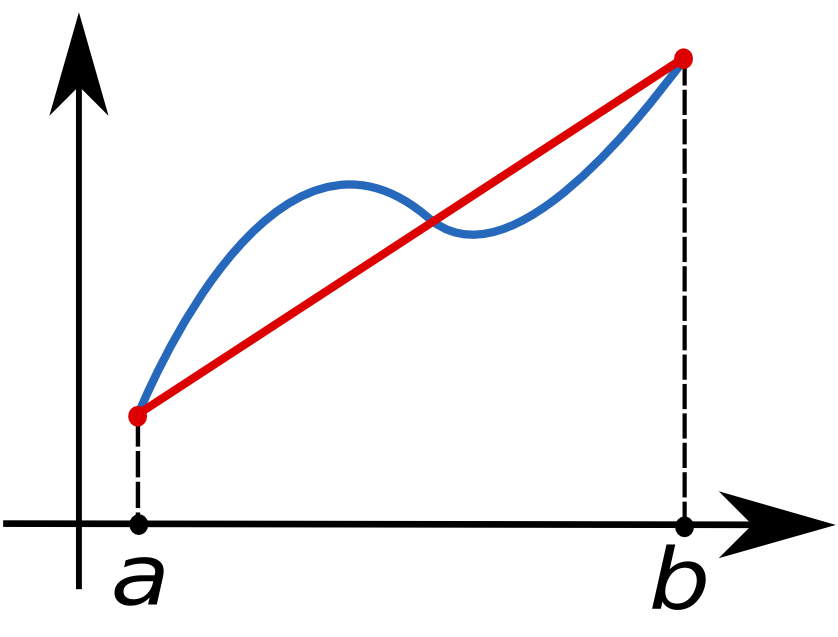
\includegraphics[scale=.15]{trapezoid.png}
\\
\\
\\
The Trapezoid Rule for approximating a definite integral is as follows:
\\
\\ $\displaystyle \int^b_a f(x)\,dx  \approx  \frac{\Delta x}{2}\Big[f(x_{0})+2f(x_1)+\ldots+2f(x_{n-1})+f(x_n)\Big]$ 
\\where \hspace{10 mm} $\displaystyle \Delta x = \frac{(b-a)}{n}$ 
\hspace{7 mm} and \hspace{7 mm} $\displaystyle x_i = a + i(\frac{b-a}{n})$
\\
\\Trapezoidal Error: 
\\
When numerically computing $\displaystyle\int^5_1x^2\,dx$, the number of intervals that are used will vary the accuracy of the calculated area. The below graphic shows the relative error ($\epsilon = \frac{\left|experimental - known\right|}{known}$) as a function of the number of intervals.
\\
\\.\hspace{10 mm} 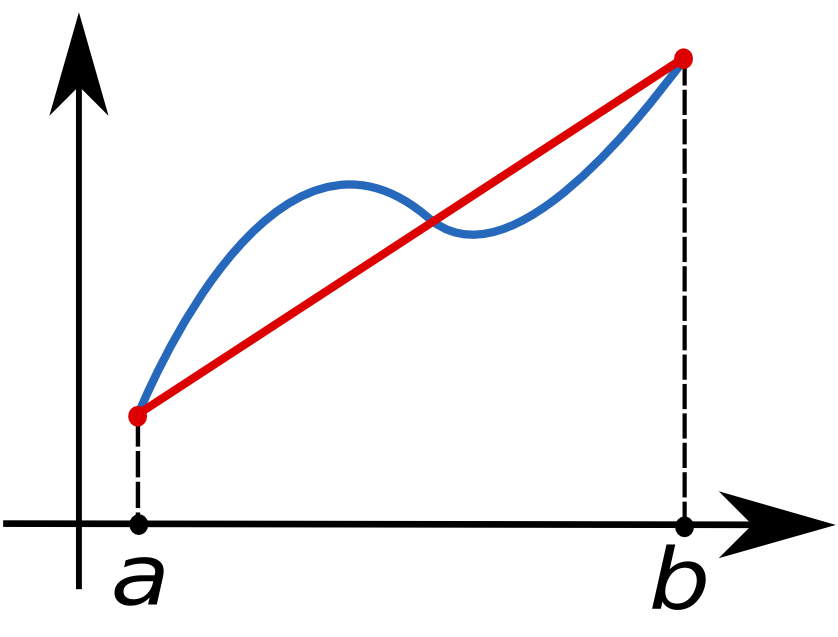
\includegraphics[scale=.95]{trapezoid.eps}
\\
\\
\\The maximum amount of truncation error ($\xi_{max_{T}}$) for the trapezoid method may be determined as follows:
\\
\\
. \hspace{20 mm} $\displaystyle \xi_{max_{T}} = \frac{(b-a)^{3}\left|f^{(2)}_{(max)}\right|}{12n^2}$ 
\\
\\
\\Here, $\displaystyle b$ and $\displaystyle a$ are the upper and lower limits of integration, $\displaystyle n$ is the number of intervals that ($b-a$) is divided into and $f^{(2)}_{(max)}$ is the second derivative of the function. The $(max)$ subscript indicates that the second derivative should be evaluated at the point from $\displaystyle [a,b]$ which maximizes the value of $f^{(2)}$.
\\
\\Similarly, the minimum number of intervals needed to approximate an integral to within a given accuracy ($\xi_{max}$) may be determined by solving the above equation for $\displaystyle n$: 
\\
. \hspace{25 mm} $\displaystyle n \geq \sqrt{\frac{(b-a)^{3}\left|f^{(2)}_{(max)}\right|}{12(\xi_{max})}} $
\\Note: $\displaystyle n$ must be a whole number; therefore if $n \geq 10.5$ then choose $n = 11$


\item Simpson's Rule:
\\
\\
Simpson's rule calculates the area under a curve much like a Riemann sum. Here, rather than using rectangles, Simpson's rule employs parabolas. The graphic below depicts the use of a red parabola between two intervals to approximate the area under the blue curve. The more intervals that are added between $a$ and $b$, the closer the "parabolic-shaped" tops of each interval will become to the tangent on the curve above it.
\\. \hspace{30 mm} 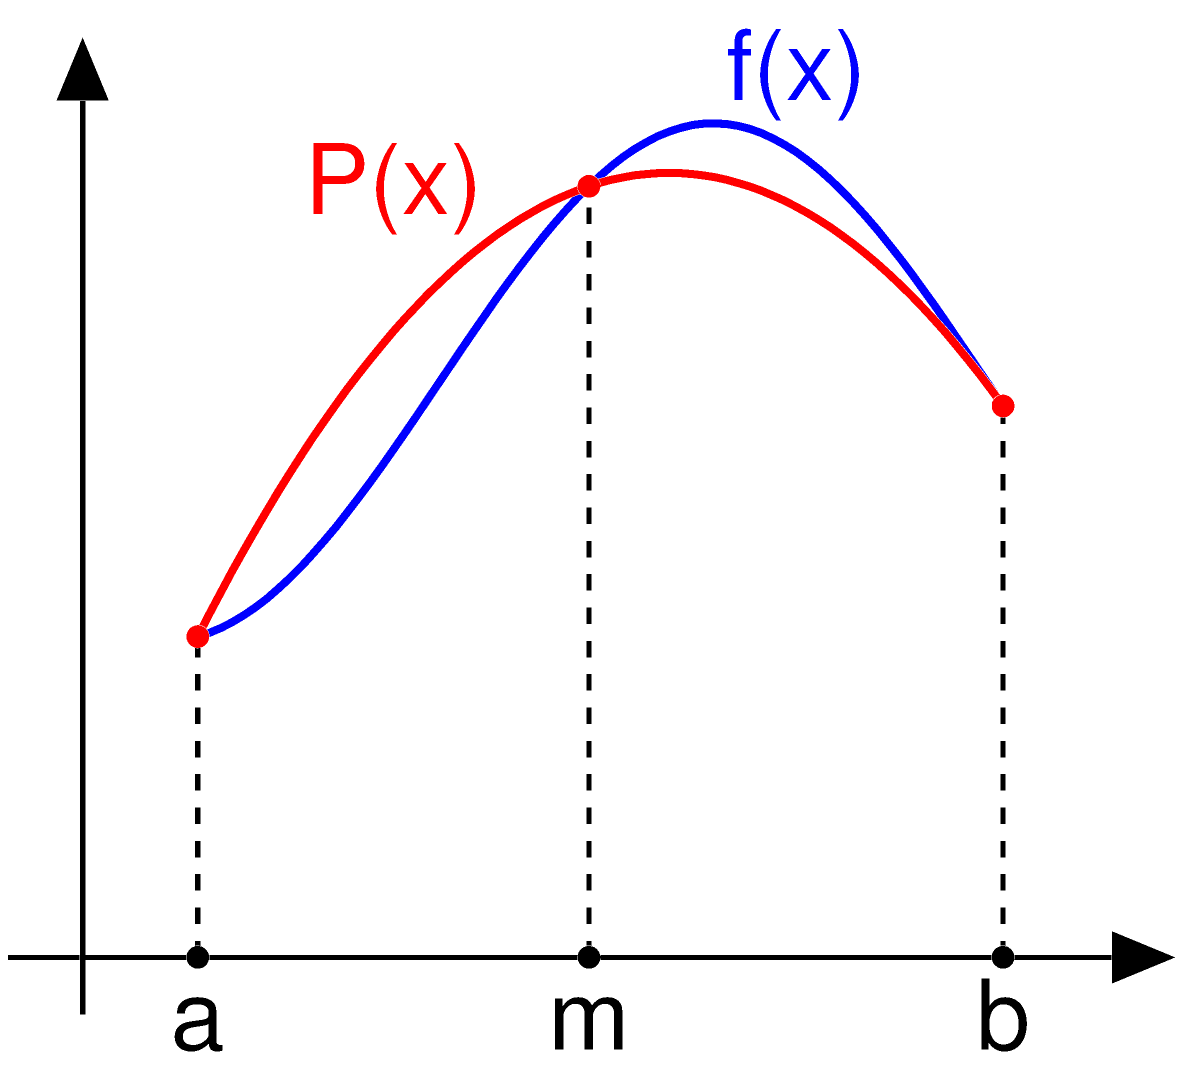
\includegraphics[scale=.10]{simpson.png}
\\
\\
The formula for calculating Simpson's Rule is as follows:
\\
\\ $\displaystyle \int^b_a f(x)\,dx  \approx  \frac{\Delta x}{3}\Big[f(x_{0})+4f(x_1)+2f(x_2)+4f(x_3)+\ldots+2f(x_{n-2})+4f(x_{n-1})+f(x_n)\Big]$, \hspace{4 mm} where $\displaystyle \Delta x = \frac{(b-a)}{n}$ 
\hspace{7 mm} and \hspace{7 mm} $\displaystyle x_i = a + i(\frac{b-a}{n})$
\\
\\Note: Simpson's Rule requires an even number of intervals $(n)$. 
\\
\\
\\
\\Simpson Rule Error: 
\\This
The accuracy of the numerical computation of $\displaystyle\int^5_1x^2\,dx$ will vary with the number of intervals used. The below graphic shows the relative error ($\epsilon$) of both Simpson's Rule (red) and the Trapezoid Method (blue). Notice how quickly Simpson's rule converges versus the Trapezoid Rule. This is largely due to Simpson's use of a parabolic curve to approximate the area under a parabola ($x^2$). Here Simpson's approximation may be exact. In the case of this quadratic function, Simpson bests Trapezoid, however, were the function linear, then the opposite would be true.
\\
\\.\hspace{10 mm} \includegraphics[scale=.95]{trapezoidsimpson.eps}
\\
\\
\\The maximum amount of truncation error ($\xi_{max_{T}}$) for Simpson's Rule may be determined as follows:
\\
\\
. \hspace{20 mm} $\displaystyle \xi_{max_{T}} = \frac{(b-a)^{5}\left|f^{(4)}_{(max)}\right|}{180n^4}$ 
\\
\\The minimum number of intervals needed to approximate an integral to within a given accuracy ($\xi_{max}$) may be determined by isolating $\displaystyle n$ from the equation above: 
\\
. \hspace{25 mm} $\displaystyle n \geq \sqrt[4]{\frac{(b-a)^{5}\left|f^{(4)}_{(max)}\right|}{180(\xi_{max})}} $
\\
\\Note: For Simpson's Rule, $\displaystyle n$ must be an even and whole number
\\
\item Three-Point Gaussian Quadrature (GQ):

Gaussian Quadrature is a numerical method of integration. Of the three methods discussed, GQ obtains the most accurate approximations or equivalent accuracy with less intervals. It does this by evaluating $f(x)$ at an abscissas which is found by determining the roots of an orthogonal polynomial of the same interval and weight. GQ is not limited to three-points, and is optimal as it can exactly fit and n-degree polynomial.
\\
\\
\\The formula for three-point Gaussian Quadrature is as follows:
\\
\\
\\$\displaystyle \int^b_a f(x)\,dx  \approx c_1f(x_1)+c_2f(x_2)+c_3f(x_3)$, where 
\\$x_1=-0.7746, x_2=0, x_3=0.7746$ and weights $c_1=0.555\overline{6}, c_2=0.888\overline{9} and c_3=0.555\overline{6}$


\end{enumerate}


\section{Numerical Differentiation Techniques}
\begin{enumerate}
\item Forward Divided Difference (FDD)
\\
\\
Forward difference is a numerical method of differentiation. It employs the limit definition of a derivative but substitutes ($\Delta x \rightarrow 0$) with a finite step size ($h$). The forward difference formula is as follows:
\\
\\
$\displaystyle f'(x) \approx \frac{f(x+\Delta x)-f(x)}{\Delta x}$ where $\Delta x$ is a finite term ($h$).
\\
\\
FDD Error:
\\
\\Because ($\Delta x \rightarrow 0$) is approximated by a finite step size ($h$), a truncation error will result. To minimize the truncation error, $h$ should be taken sufficient small. However, there is a computational limit to how small $h$ may be. Machine Epsilon ($\epsilon$) is the largest number that when added to another number, does not change it. This number is specific to both the systems architecture and the data structure storing the number. In my case, my machine epsilon ($\epsilon$) for a double is $2.2204460492503131\times10^-16$. If $h$ is chosen to be $\geq \epsilon$ then $\xi_{max}$ will be $\geq 1$. Therefore, to minimize error, and thereby maximize accuracy, an $h$ should be chosen such that the truncation error and round-off error or approximately the same.
\\
\\The following $LogLog$-plot depicts the relative error($\epsilon$) versus step size ($h$) of the FDD approximations for: $x^2(blue)$, $x^3(red)$, $e^{-x}(green)$ and $sin(x)ln(x)(brown)$
\\
\\
\\.\hspace{6 mm} 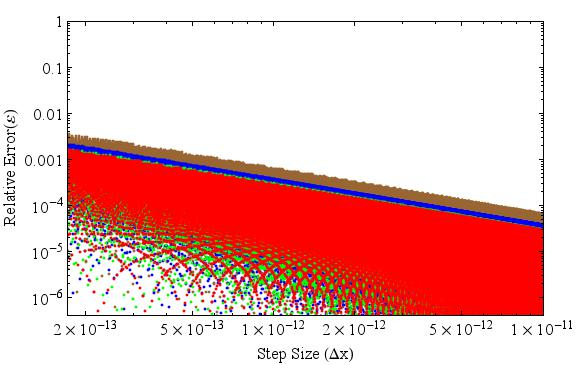
\includegraphics[scale=.5]{forwardDiff.jpeg}
\\
\\
\\
\item Central Divided Difference (CDD)
\\
\\The Central Difference is similar to FDD except that CDD is evaluated at half of the step size. Due to this, CDD has an additional order of accuracy for smooth functions. The Central Fifference formula is as follows:
\\
\\
\\$\displaystyle f'(x) \approx \frac{f(x+\Delta x)-f(x)}{2\Delta x}$ where $\Delta x$ is a finite term ($h$).
\\
\\
\\\\The following $LogLog$-plot depicts the relative error($\epsilon$) versus step size ($h$) of the CDD approximations for: $x^2(blue)$, $x^3(red)$, $e^{-x}(green)$ and $sin(x)ln(x)(brown)$
\\
\\.\hspace{6 mm} 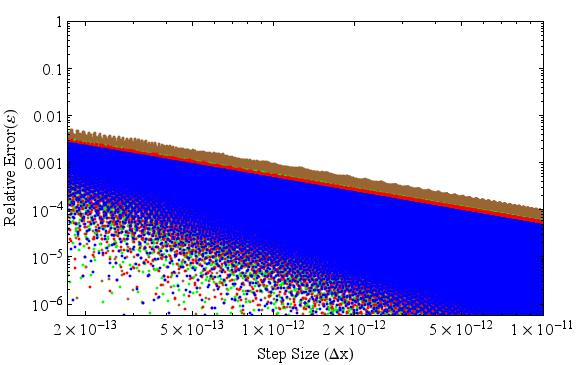
\includegraphics[scale=.5]{centralDiff.jpeg}
\item Five Point Stencil (FPS)y
\\The formula for the FPS method is as follows:
\\
\\$\displaystyle f'(x) \approx \frac{-f(x+\Delta x)+8f(x+\Delta x)-8f(x-\Delta x)+f(x-2\Delta x)}{12\Delta x}$ 
\\where $\Delta x$ is a finite term ($h$).
\\
\\Truncation error due to the FPS may be estimated as follows:
\\
\\.\hspace{25 mm}$\xi_{max} = f'(x)-\frac{1}{30}f^5(x)h^4+O(h^5)$
\\\\The following $LogLog$-plot depicts the relative error($\epsilon$) versus step size ($h$) of the FPS approximations for: $x^2(blue)$, $x^3(red)$, $e^{-x}(green)$ and $sin(x)ln(x)(brown)$
\\\\.\hspace{6 mm} 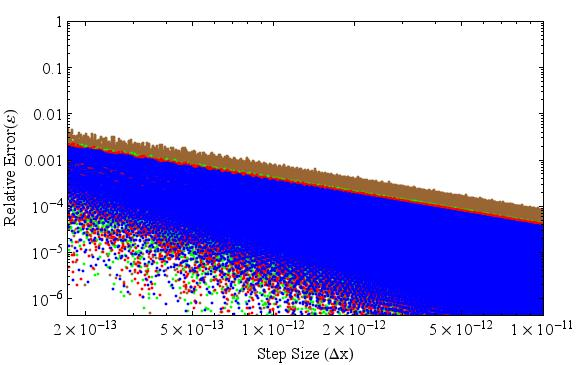
\includegraphics[scale=.5]{fivePoint.jpeg}
\end{enumerate}


\end{document}
